% =============================================================================
% mass-energy-balance-flow.tex — Sankey-style mass balance for a conversion
% process: one feedstock stream in, three product streams out, with mass %
% labels. Adapt stream count/labels for your process.
%
% Compiles standalone via: xelatex mass-energy-balance-flow.tex
% =============================================================================

\documentclass[border=4pt]{standalone}
\usepackage{tikz}
\usetikzlibrary{arrows.meta, positioning}

\definecolor{node-fill}{HTML}{E8EDF5}
\definecolor{node-border}{HTML}{012169}
\definecolor{stream-color}{HTML}{012169}
\definecolor{label-color}{HTML}{1A1A1A}

\tikzset{
  process-node/.style={
    draw=node-border, fill=node-fill, rounded corners=2pt,
    minimum width=2.8cm, minimum height=1.2cm, align=center, font=\small
  },
  stream/.style={-{Latex[length=3mm]}, line width=1.2pt, draw=stream-color}
}

% -----------------------------------------------------------------------------
% Diagram: Feedstock -> Reactor -> {Biochar, Bio-oil, Syngas}, mass % labeled.
% Coordinates (center of each node):
%   feedstock at (0,    0)
%   reactor   at (3.5,  0)
%   biochar   at (7.5,  1.8)
%   biooil    at (7.5,  0)
%   syngas    at (7.5, -1.8)
% Reactor is 2.8cm wide (half-width 1.4cm); output nodes start at x=6.1,
% clearing the reactor's right edge (x=4.9) by 1.2cm.
% -----------------------------------------------------------------------------

\begin{document}
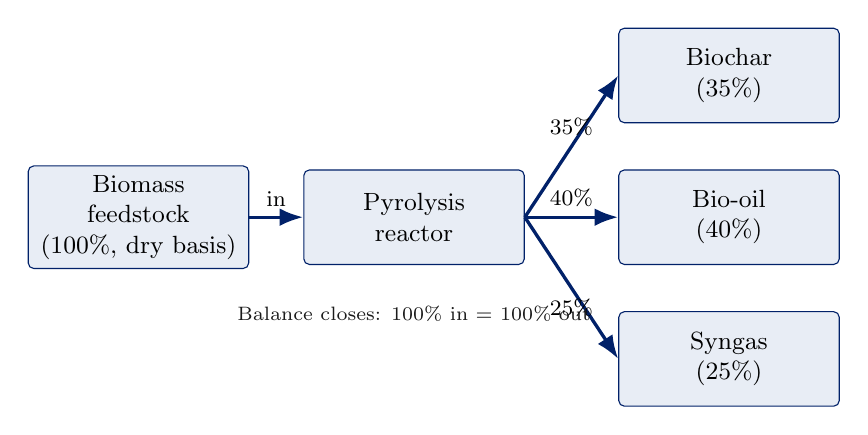
\begin{tikzpicture}
  \node[process-node] (feedstock) at (0, 0)    {Biomass\\feedstock\\(100\%, dry basis)};
  \node[process-node] (reactor)   at (3.5, 0)  {Pyrolysis\\reactor};
  \node[process-node] (biochar)   at (7.5, 1.8) {Biochar\\(35\%)};
  \node[process-node] (biooil)    at (7.5, 0)   {Bio-oil\\(40\%)};
  \node[process-node] (syngas)    at (7.5, -1.8){Syngas\\(25\%)};

  \draw[stream] (feedstock) -- node[midway, above] {\footnotesize in} (reactor);
  \draw[stream] (reactor.east) -- node[midway, above] {\footnotesize 35\%} (biochar.west);
  \draw[stream] (reactor.east) -- node[midway, above] {\footnotesize 40\%} (biooil.west);
  \draw[stream] (reactor.east) -- node[midway, below] {\footnotesize 25\%} (syngas.west);

  % Mass-balance closure note — replace with the actual closure check.
  \node[font=\scriptsize, text=label-color, below=0.4cm of reactor] {Balance closes: 100\% in = 100\% out};
\end{tikzpicture}
\end{document}
